\documentclass[11pt]{article}
\usepackage{fullpage}
\usepackage{float}
\usepackage{graphicx}
\usepackage{amssymb}
\usepackage{subcaption}
\usepackage{mwe}
\usepackage{epstopdf}
\usepackage{color,verbatim}
\usepackage{bm}
\usepackage{listings}
\usepackage{mathtools}          %loads amsmath as well
\usepackage{titling}
\DeclareGraphicsRule{.tif}{png}{.png}{`convert #1 `dirname #1`/`basename #1 .tif`.png}
%\usepackage{doublespace}

\begin{document}
\title{Weekly Status Report}
\author{Development of a 1D Adaptive Wavelet Collocation Code \\
Brandon Gusto \\}
\date{Week Beginning 8/21/03}

\maketitle
%
\section{Summary of efforts from last week}
\begin{enumerate}
    \item Completed codes to construct second-generation interpolating wavelets. Both the scaling functions 
        $\phi_{m}^{J}(x)$ and the detail wavelet functions $\psi_{m}^{J}(x)$ can be constructed to an 
        arbitrarily high level of resolution, $J$. This is done using the interpolating subdivision scheme based on Deslauriers \& Dubuc 1989.
    \item Investigated binary search tree algorithms for dynamic allocation of dyadic grid information.  
\end{enumerate}
\begin{figure*}
    \centering
    \begin{subfigure}[b]{0.475\textwidth}
        \centering
        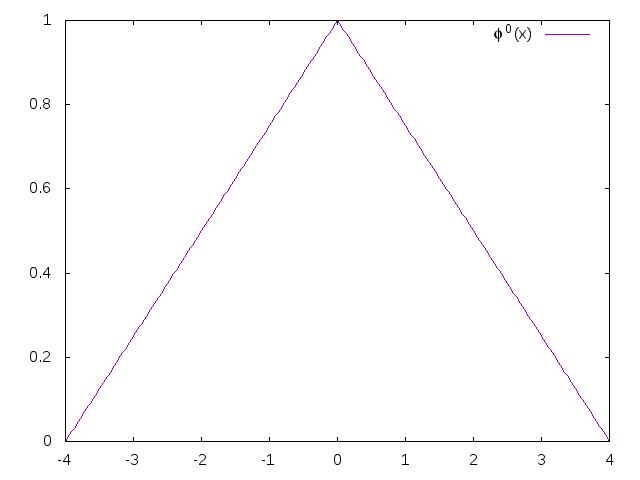
\includegraphics[width=\textwidth]{../../../../Programs/Wavelet/1D_Burger/AWCM/src/output/scaling_j0.png}
        \caption[Network2]%
        {{\small $j=0$}}    
    \end{subfigure}
    \hfill
    \begin{subfigure}[b]{0.475\textwidth}  
        \centering 
        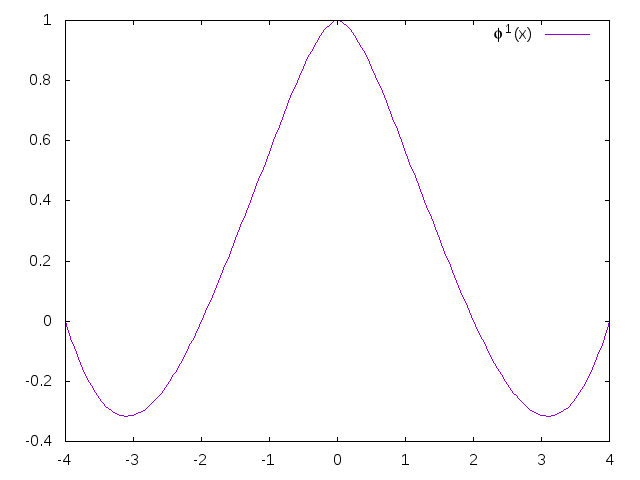
\includegraphics[width=\textwidth]{../../../../Programs/Wavelet/1D_Burger/AWCM/src/output/scaling_j1.png}
        \caption[]%
        {{\small $j=1$}}    
    \end{subfigure}
    \vskip\baselineskip
    \begin{subfigure}[b]{0.475\textwidth}   
        \centering 
        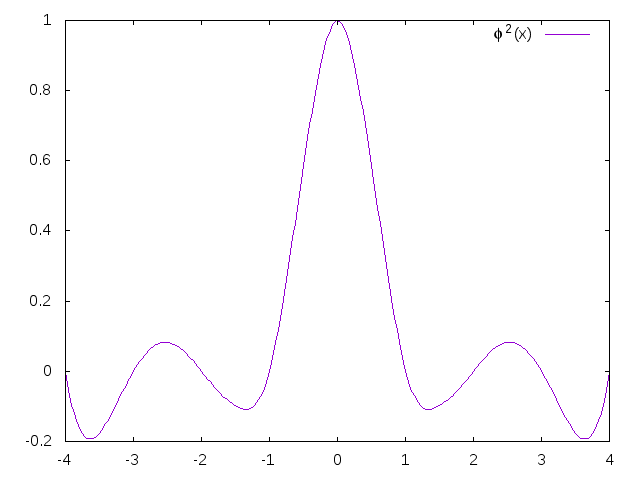
\includegraphics[width=\textwidth]{../../../../Programs/Wavelet/1D_Burger/AWCM/src/output/scaling_j2.png}
        \caption[]%
        {{\small $j=2$}}    
    \end{subfigure}
    \quad
    \begin{subfigure}[b]{0.475\textwidth}   
        \centering 
        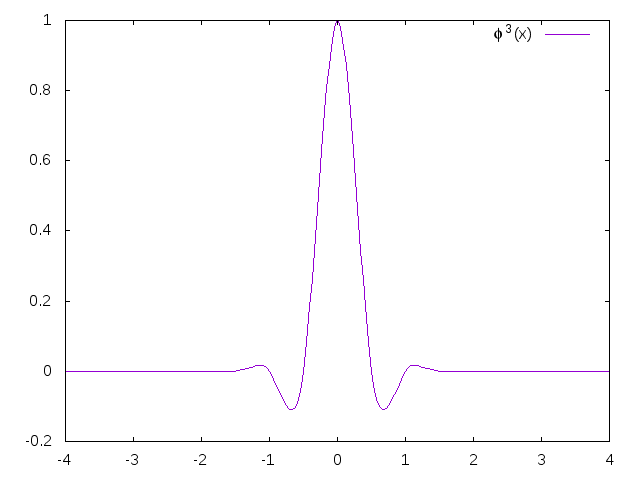
\includegraphics[width=\textwidth]{../../../../Programs/Wavelet/1D_Burger/AWCM/src/output/scaling_j3.png}
        \caption[]%
        {{\small $j=3$}}    
    \end{subfigure}
    \caption[ The average and standard deviation of critical parameters ]
    {{\small Scaling functions $\phi (x)$ for various levels $j$.}} 
    \label{fig:mean and std of nets}
\end{figure*}
\begin{figure}[H]
    \center
    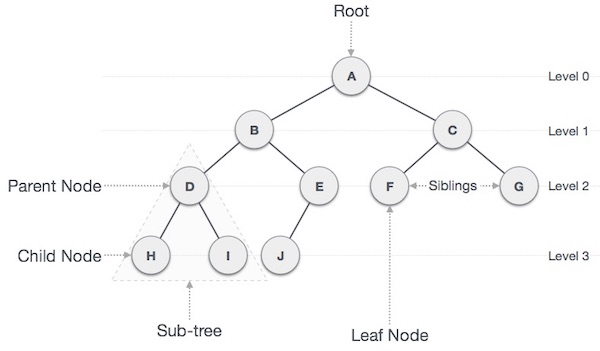
\includegraphics[scale=0.5]{../image/binary_tree.jpg}
\end{figure}

\begin{figure*}
    \centering
    \begin{subfigure}[b]{0.475\textwidth}
        \centering
        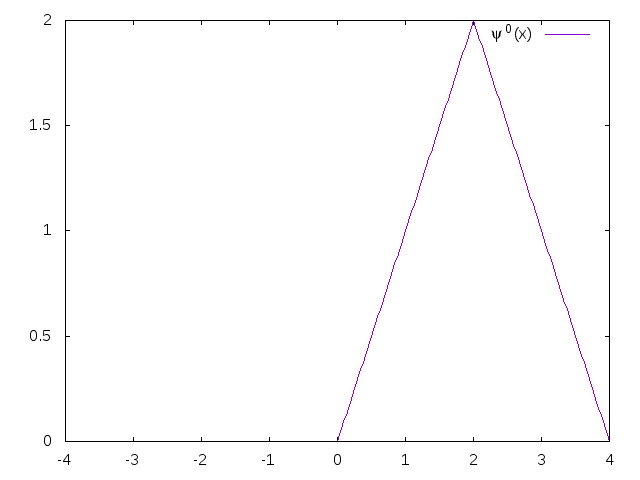
\includegraphics[width=\textwidth]{../../../../Programs/Wavelet/1D_Burger/AWCM/src/output/detail_j0.png}
        \caption[Network2]%
        {{\small $j=0$}}    
    \end{subfigure}
    \hfill
    \begin{subfigure}[b]{0.475\textwidth}  
        \centering 
        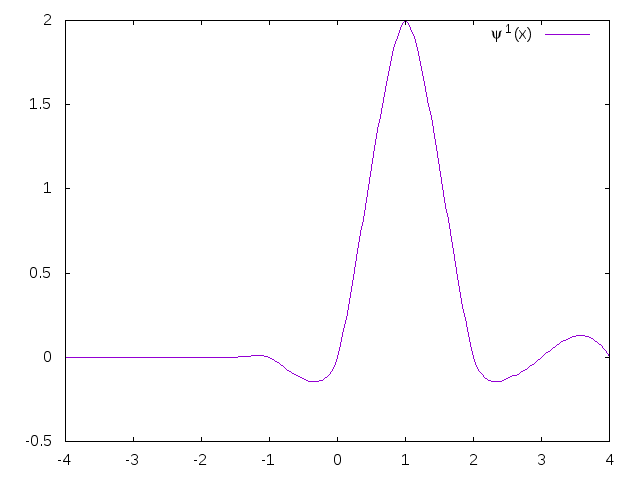
\includegraphics[width=\textwidth]{../../../../Programs/Wavelet/1D_Burger/AWCM/src/output/detail_j1.png}
        \caption[]%
        {{\small $j=1$}}    
    \end{subfigure}
    \vskip\baselineskip
    \begin{subfigure}[b]{0.475\textwidth}   
        \centering 
        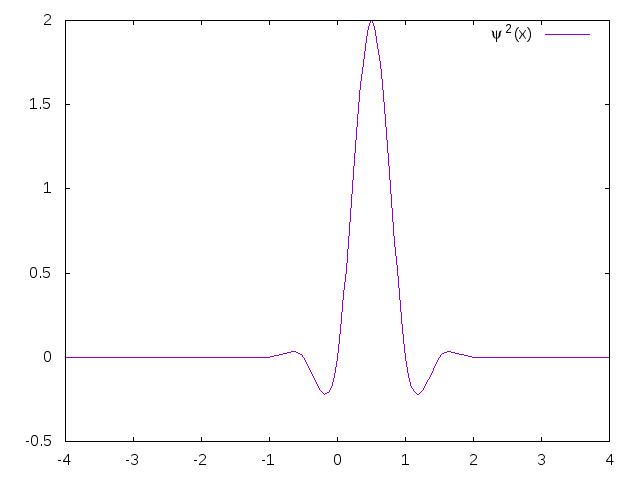
\includegraphics[width=\textwidth]{../../../../Programs/Wavelet/1D_Burger/AWCM/src/output/detail_j2.png}
        \caption[]%
        {{\small $j=2$}}    
    \end{subfigure}
    \quad
    \begin{subfigure}[b]{0.475\textwidth}   
        \centering 
        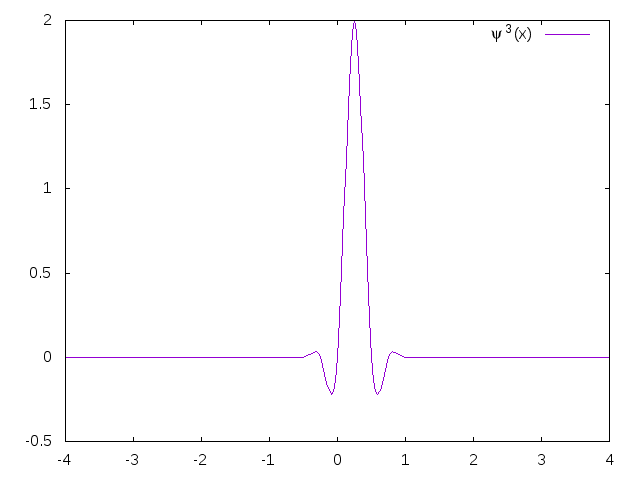
\includegraphics[width=\textwidth]{../../../../Programs/Wavelet/1D_Burger/AWCM/src/output/detail_j3.png}
        \caption[]%
        {{\small $j=3$}}    
    \end{subfigure}
    \caption[ The average and standard deviation of critical parameters ]
    {{\small Daughter wavelet functions $\psi (x)$ for various levels $j$.}} 
    \label{fig:mean and std of nets}
\end{figure*}
%
\section{This week's goals}
\begin{enumerate}
\item To use the scaling and detail wavelet functions, in conjunction with the forward wavelet transform, to approximate some initial function 
    $u(x)$. A function $u(x)$ may be approximated by
    \begin{equation}
        u^J(x)=\sum_{k \in \mathcal{K^0}} c_{k}^{0} \phi_{k}^{0}(x) + \sum_{j=0}^{J-1} \sum_{l \in \mathcal{L}^j}
                d_{l}^{j} \psi_{l}^{j}(x).
    \end{equation}
\item Once a function can be approximated, an algorithm to throw away small detail coefficients can be developed.
\item The grid points can then be altered using the binary tree structure.
\item Develop a code to calculate spatial derivatives as in Vasilyev \& Bowman (2000).
\end{enumerate}

\end{document}
